


\usetikzlibrary{calc}




\newcommand{\drawgrid}[5][]{%
\draw[line cap=rect,#1] (#2,#3) grid ++ (#4,#5); 
}

\newcommand{\drawrect}[5][]{%
\draw[line cap=rect,#1] (#2,#3) rectangle ++ (#4,#5); 
}


\newcommand{\fillcoord}[2]{%
\fill[black] (#1,#2) rectangle ++ (1,1); 
}

\newcommand{\namecoord}[4]{%
\node[label=center:#4] (#3) at ($(#1,#2)+(0.5,0.5)$) {}; 
}


\newcommand{\selectcoord}[2]{%
\draw[color=red, line width=1pt, line cap=rect]  (#1,#2) grid ($(#1,#2)+(1,1)$) {}; 
}

\newcommand{\linkcoord}[5][]{%
\draw[->,color=red, line width=1pt, line cap=rect,#1]  ($(#2,#3)+(0.5,0.5)$) -- ($(#4,#5)+(0.5,0.5)$) {}; 
}





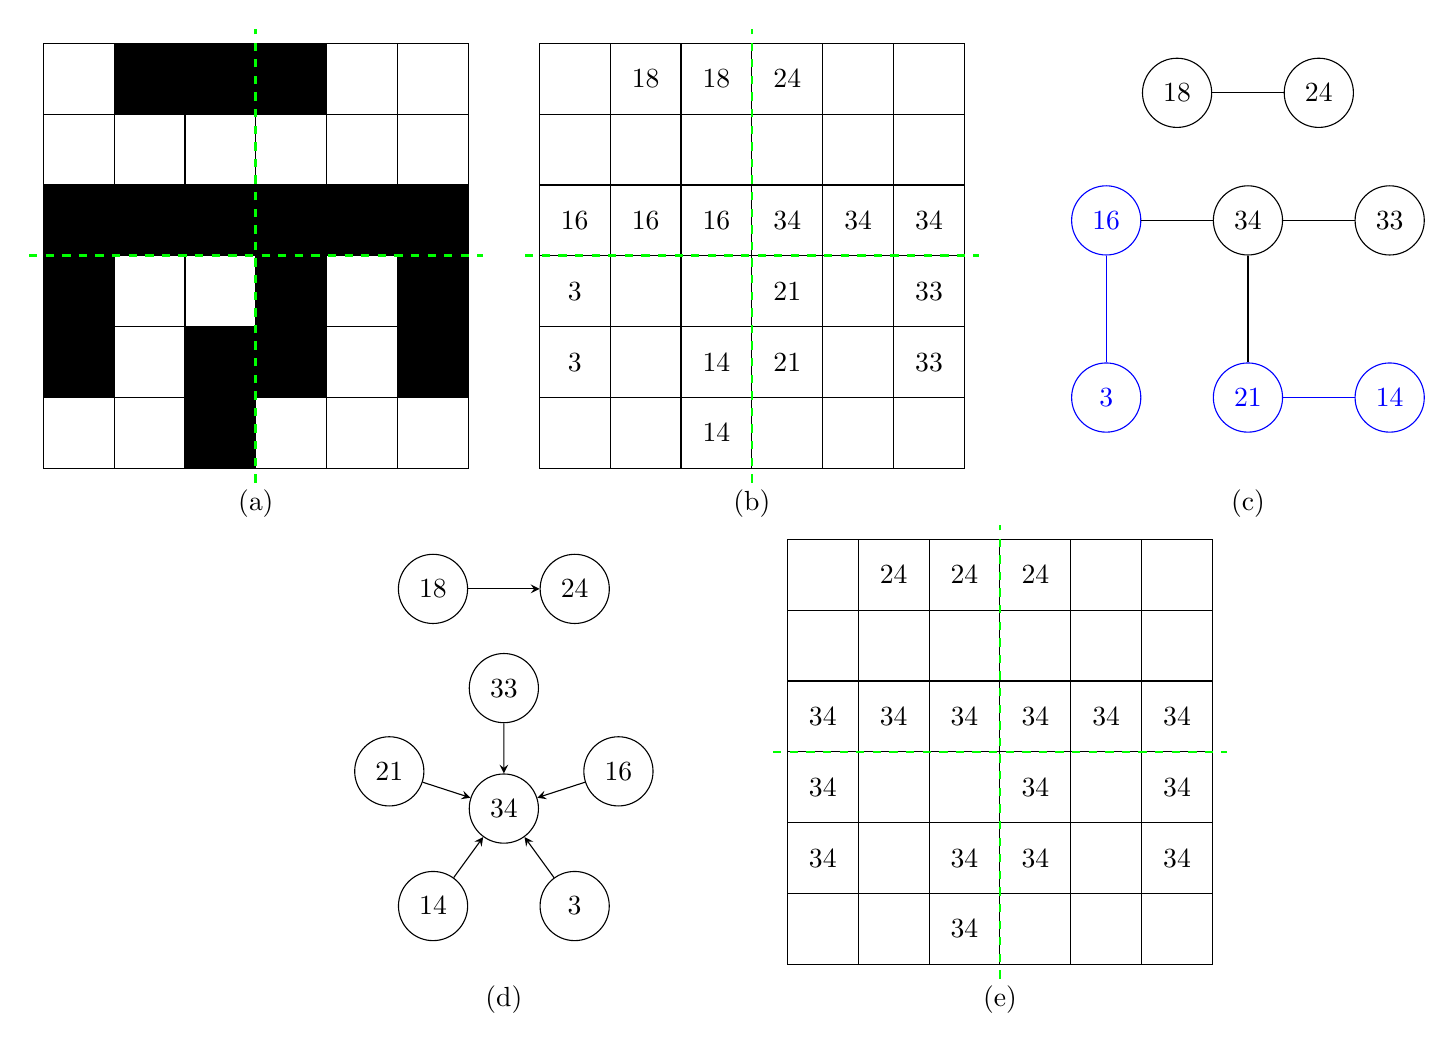
\begin{tikzpicture}[scale=0.9]


\begin{scope}[shift={(0,0)}]
\namecoord{2.5}{-1}{}{(a)}


\drawgrid{0}{0}{6}{6}

% bloc 00
\fillcoord{0}{1}
\fillcoord{0}{2}

\fillcoord{2}{1}
\fillcoord{2}{0}

% bloc 01
\fillcoord{1}{5}
\fillcoord{2}{5}

\fillcoord{0}{3}
\fillcoord{1}{3}
\fillcoord{2}{3}

% bloc 11
\fillcoord{3}{5}

\fillcoord{3}{3}
\fillcoord{4}{3}
\fillcoord{5}{3}

% bloc 10
\fillcoord{5}{2}
\fillcoord{5}{1}

\fillcoord{3}{2}
\fillcoord{3}{1}



\draw[dashed,green,line width=1pt] (3,-0.2) -- (3,6.2);
\draw[dashed,green,line width=1pt] (-0.2,3) -- (6.2,3);
\end{scope}

\begin{scope}[shift={(7,0)}]
\namecoord{2.5}{-1}{}{(b)}


\drawgrid{0}{0}{6}{6}

% bloc 00
\namecoord{0}{1}{}{3}
\namecoord{0}{2}{}{3}

\namecoord{2}{1}{}{14}
\namecoord{2}{0}{}{14}

% bloc 01
\namecoord{1}{5}{}{18}
\namecoord{2}{5}{}{18}

\namecoord{0}{3}{}{16}
\namecoord{1}{3}{}{16}
\namecoord{2}{3}{}{16}

% bloc 11
\namecoord{3}{5}{}{24}

\namecoord{3}{3}{}{34}
\namecoord{4}{3}{}{34}
\namecoord{5}{3}{}{34}

% bloc 10
\namecoord{5}{2}{}{33}
\namecoord{5}{1}{}{33}

\namecoord{3}{2}{}{21}
\namecoord{3}{1}{}{21}



\draw[dashed,green,line width=1pt] (3,-0.2) -- (3,6.2);
\draw[dashed,green,line width=1pt] (-0.2,3) -- (6.2,3);
\end{scope}

\begin{scope}[shift={(14,0)}]
\namecoord{2.5}{-1}{}{(c)}


% \drawrect{0}{0}{6}{6}

\tikzstyle{graphnode}=[draw,circle,minimum size=25pt]
\node[graphnode] (g18) at (2,5.3) {18};
\node[graphnode] (g24) at (4,5.3) {24};

\draw (g18) -- (g24);

\node[graphnode,blue] (g3) at (1,1) {3};
\node[graphnode,blue] (g16) at (1,3.5) {16};
\node[graphnode] (g34) at (3,3.5) {34};
\node[graphnode] (g33) at (5,3.5) {33};
\node[graphnode,blue] (g21) at (3,1) {21};
\node[graphnode,blue] (g14) at (5,1) {14};

\draw[blue] (g3) -- (g16);
\draw (g34) -- (g16);
\draw (g34) -- (g33);
\draw (g34) -- (g21);
\draw[blue] (g14) -- (g21);
\end{scope}

\begin{scope}[shift={(3.5,-7)}]
\namecoord{2.5}{-1}{}{(d)}


% \drawrect{0}{0}{6}{6}

\tikzstyle{graphnode}=[draw,circle,minimum size=25pt]
\node[graphnode] (g18) at (2,5.3) {18};
\node[graphnode] (g24) at (4,5.3) {24};

\draw[-stealth] (g18) -- (g24);

\node[graphnode] (g34) at (3,2.2) {34};

\def\startangle{-54}
\def\nodedistance{1.7}
\node[graphnode] (g3) at ($(g34)+(\startangle:\nodedistance)$) {3};
\node[graphnode] (g16) at ($(g34)+(\startangle+72:\nodedistance)$) {16};

\node[graphnode] (g33) at ($(g34)+(\startangle+144:\nodedistance)$) {33};
\node[graphnode] (g21) at ($(g34)+(\startangle+216:\nodedistance)$) {21};
\node[graphnode] (g14) at ($(g34)+(\startangle+288:\nodedistance)$) {14};

\draw[-stealth] (g3) -- (g34);
\draw[-stealth] (g16) -- (g34);
\draw[-stealth] (g33) -- (g34);
\draw[-stealth] (g21) -- (g34);
\draw[-stealth] (g14) -- (g34);
\end{scope}

\begin{scope}[shift={(10.5,-7)}]
\namecoord{2.5}{-1}{}{(e)}


\drawgrid{0}{0}{6}{6}

% bloc 00
\namecoord{0}{1}{}{34}
\namecoord{0}{2}{}{34}

\namecoord{2}{1}{}{34}
\namecoord{2}{0}{}{34}

% bloc 01
\namecoord{1}{5}{}{24}
\namecoord{2}{5}{}{24}

\namecoord{0}{3}{}{34}
\namecoord{1}{3}{}{34}
\namecoord{2}{3}{}{34}

% bloc 11
\namecoord{3}{5}{}{24}

\namecoord{3}{3}{}{34}
\namecoord{4}{3}{}{34}
\namecoord{5}{3}{}{34}

% bloc 10
\namecoord{5}{2}{}{34}
\namecoord{5}{1}{}{34}

\namecoord{3}{2}{}{34}
\namecoord{3}{1}{}{34}



\draw[dashed,green,line width=1pt] (3,-0.2) -- (3,6.2);
\draw[dashed,green,line width=1pt] (-0.2,3) -- (6.2,3);
\end{scope}


\end{tikzpicture}



